\chapter{Appendix}
\section{Inlist files from MESA and GYRE}
\label{inlist}

\subsection{MESA inlist}

The standard inlist file used in \texttt{MESA} grid construction for this work is shown here. The \texttt{initial\_h1},\texttt{initial\_he3},\texttt{initial\_he4}, \texttt{mixing\_length\_alpha}, \texttt{new\_mass} and the different \texttt{step\_overshoot\_f} commands changes the values of $X,Z,M,\alpha_{mlt},\alpha_{ov}$ respectively. This is done through a bash script searching and replacing the correct values. 

\lstinputlisting[language=Fortran]{appendix_stuff/inlist_premainmade}

\subsection{GYRE input file to output}

This section shows a bash script which creates an inlist file to run GYRE on a profiles.data.GYRE output file, and create an output file. This code has the option to call radial orders only.
\lstinputlisting[language=Bash]{appendix_stuff/gyre_tofreqs_44tau.sh}

\section{\chis routine}
\label{chisroutine}

For the purpose of calculating the \chis, multiple codes are used. Here, only some of them are presented. All files used in this project can be seen on the webpage \url{https://github.com/JanneMon/Thesis-codes}. 

First, all profiles for all tracks located in the grid directory (\texttt{output\_smallgrid}) are read into \texttt{call\_chi.py} which is the main file. This calls several files (not listed here) to extract input parameters, observational properties and pulsations.  A file with all the information is created for each track and put into a separate directory \texttt{Results\_l0}\footnote{The "l0" indicates that the luminosity comes from the first dataset}. 

\lstinputlisting[language=python]{appendix_stuff/call_chi.py}

This also does call an initially used \chis code \texttt{calculate\_chis\_ff1.py} which was implemented wrong and resulted in $\chi_{freqs}=1$. Therefore, the correct \chis test used in this project is conducted in a separate file \texttt{call\_chi\_actually} that takes the output files in the \texttt{Results\_l0} directory, calculates the \chis based on the observational and pulsational values in the file and creates a new results file in \texttt{new\_Results\_l0}. 

\lstinputlisting[language=python]{appendix_stuff/call_chi_actually.py}

The output files created contains all \chis information $\chi_{tot}^2$,$\chi_{freqs}^2$, $\chi_{obs}^2$ and the artificially pumped total \chis and frequencies $\chi_{p}^2$, $\chi_{freqs,p}^2$. For each file (containing information for an entire track) the lowest $\chi_{ tot}^2$ is found. Among these, the best 5\% models are found. These selections happens in \texttt{plot\_chis\_actually.py}:

\lstinputlisting[language=python]{appendix_stuff/plot_chis_actually.py}

This will create an ouput file with the names of the 5\% best models, as listed in \tabref{bestchi_m1}. It also produces a plot with the best \chis model for each track plotted as a function of mass. An example plot can be seen on \figref{selectfive}. 

\begin{figure}[htbp]
	\centering
	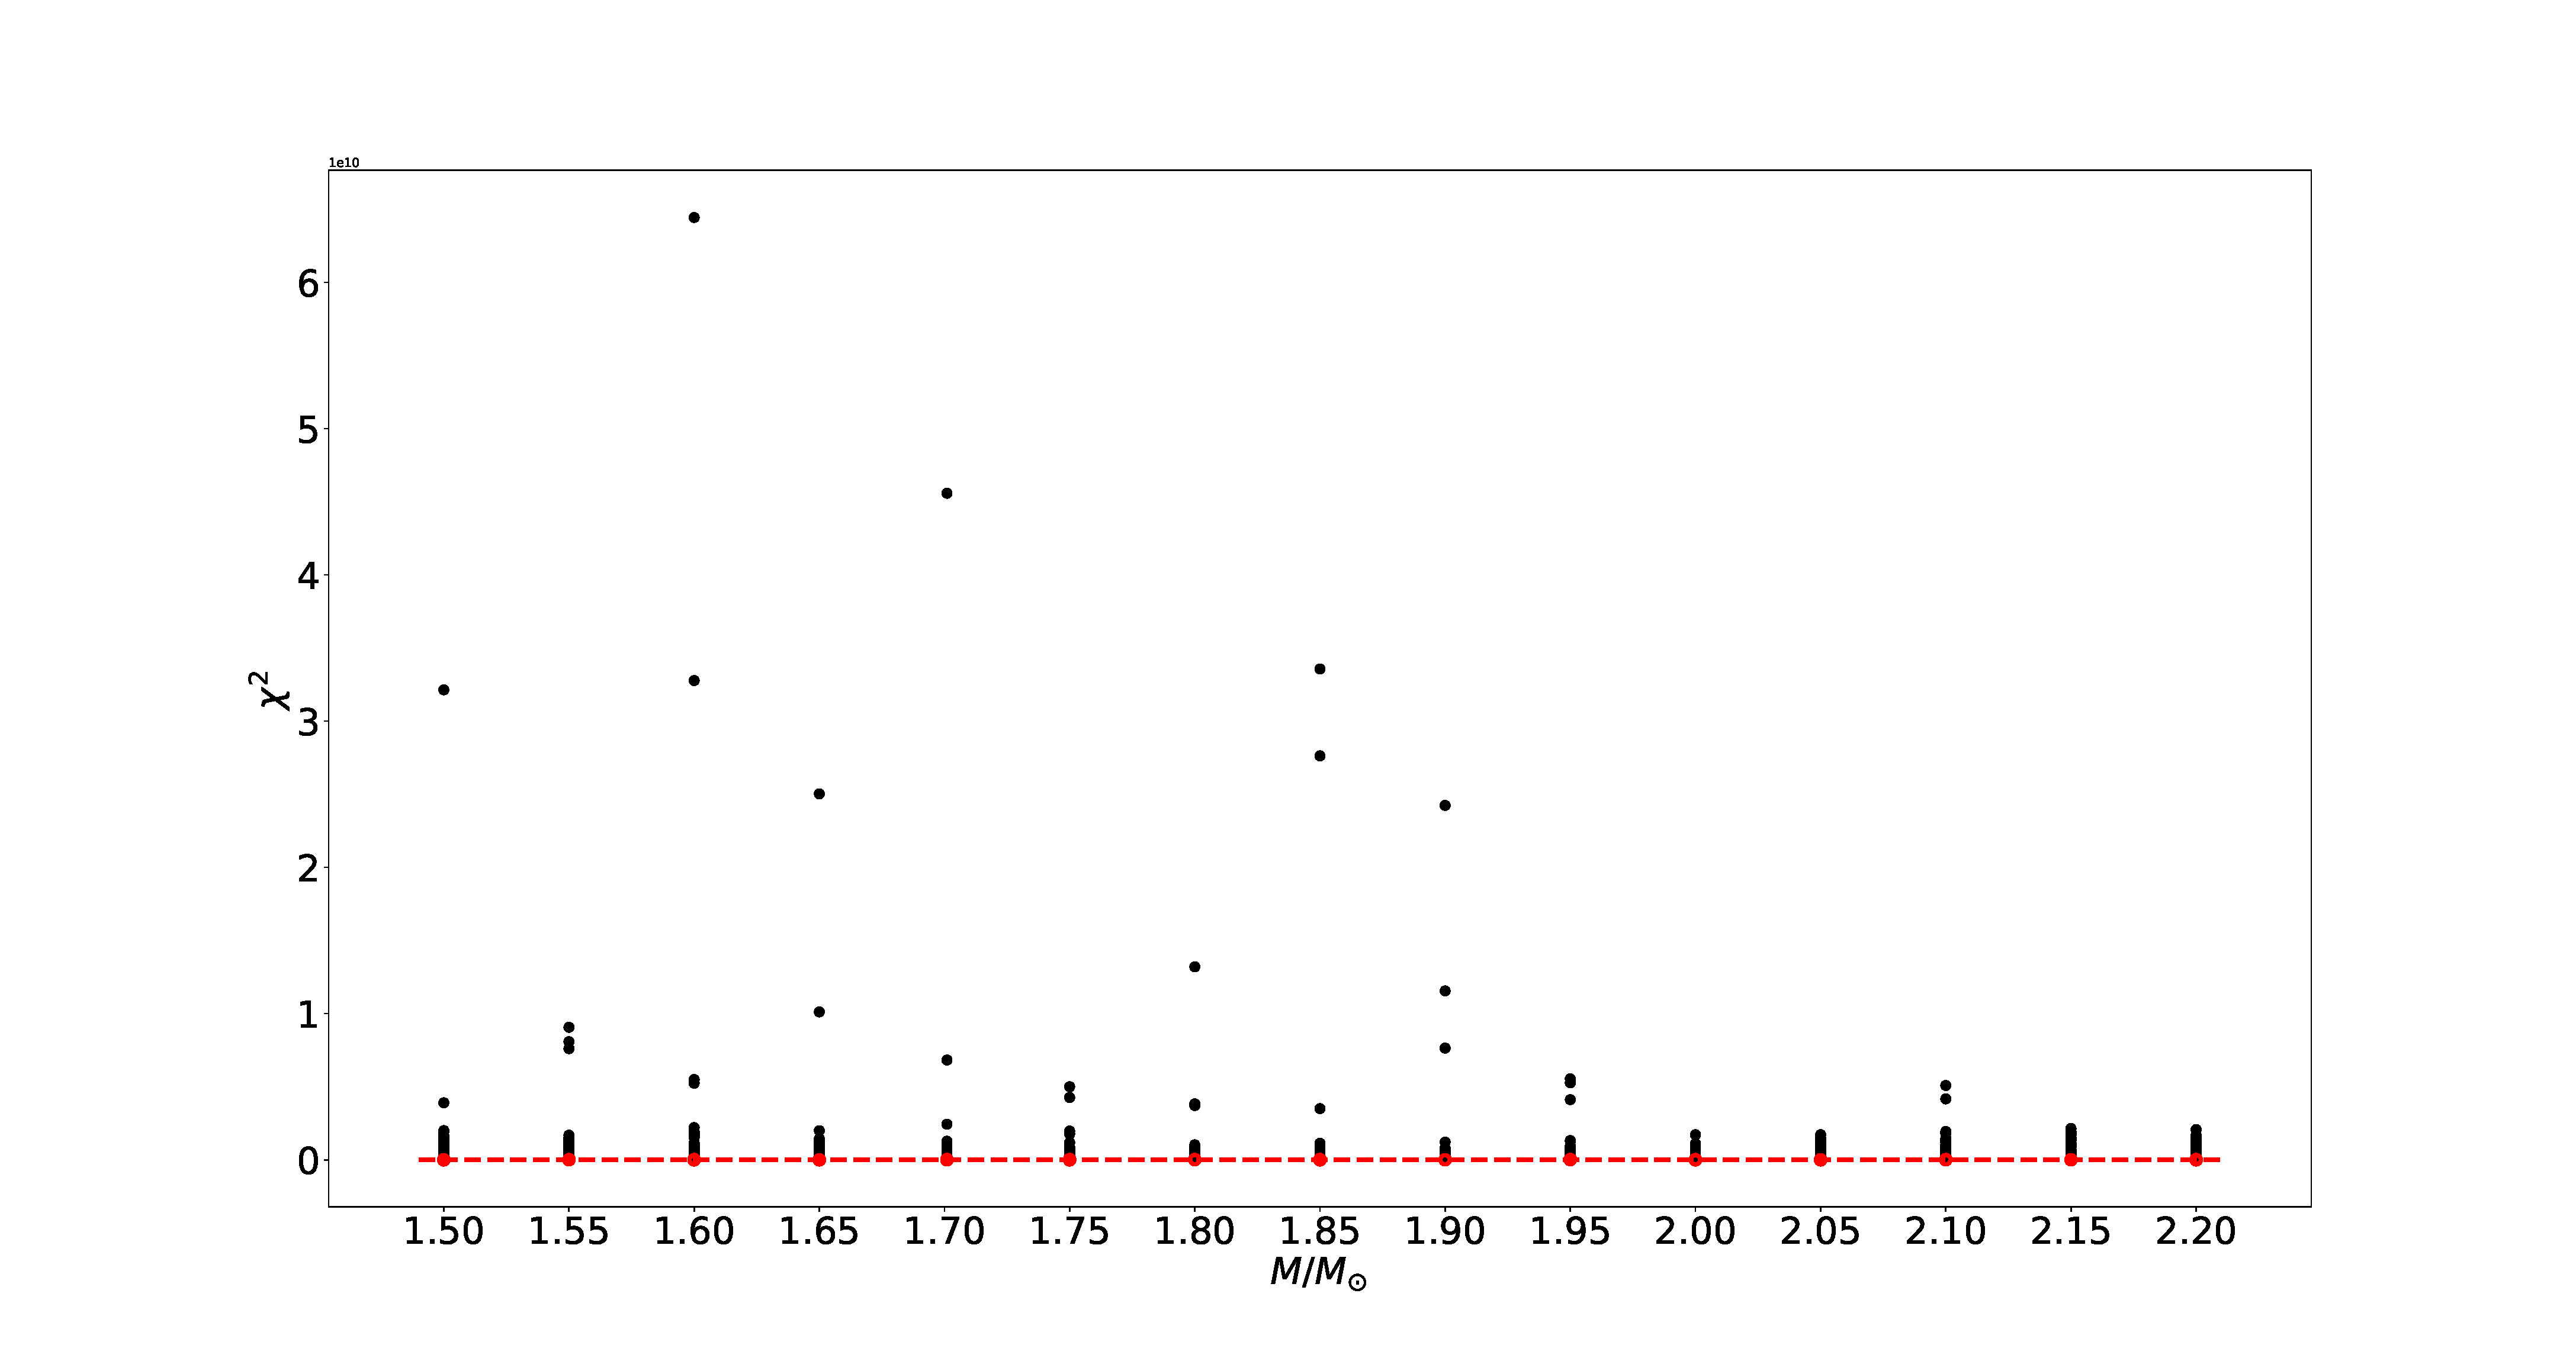
\includegraphics[width=1\textwidth]{appendix_stuff/plotchis.eps}
	\caption{Lowest \chis models for each track plotted as a function of mass. The red lines indicates the 5\% lower \chis limit for models to be included into the best 5\%.   }
	\label{selectfive}
\end{figure}

The non-radial pulsations are then calculated in \texttt{GYRE} for the 5\% best models. From these, the \chis routine for $l=0,1,2$ is run to obtain new \chis. This is done in \texttt{getl1l2\_results\_actually\_version2.py}

\lstinputlisting[language=python]{appendix_stuff/getl1l2_actually.py},

\noindent which produces the final output file. This file is then opened in \texttt{test\_l012\_results\_actually\_version2.py}.

\lstinputlisting[language=python]{appendix_stuff/test_l012_results_actually_version2.py},

 The output prints the minimum  $\chi_{tot}^2$,  $\chi_{obs}^2$, $\chi_{freqs}^2$  and $\chi_{p}^2$ (enhanced total \chis). All of these routines are for 44 Tau calculations. The routines for HD 187547 are similar, but with different directories. The \chis code also implements a routine for calculating the separation. This is done in \texttt{calculate\_chis\_ff1\_superstar\_withcorrectsep.py} called in the main file which is similar to the main file for 44 Tau, and is therefore not listed here).
 
\lstinputlisting[language=python]{appendix_stuff/calculate_chis_ff1_superstar_withcorrectsep.py}. 
 
 

